\RequirePackage{plautopatch}
\documentclass[dvipdfmx]{jsarticle}
%
\input preamble.tex

%
\title{モナド}
\author{ぱて(@pte\_hs)}
\date{\today}
\begin{document}
\maketitle
% 
%

\section{まえがき}
LaTeXの練習を兼ねて,最近学んでいるモナドについて整理しようと考えた.

\section{定義}
\begin{dfn}[モナド]
モナド$\ \langle T, \eta, \mu \rangle $とは,自己関手$T: X \to X$, 自然変換 $\eta: I \to T$, $\mu: T \times T \to T$の組であり,
次の図式を可換にするものである.\\ \\
  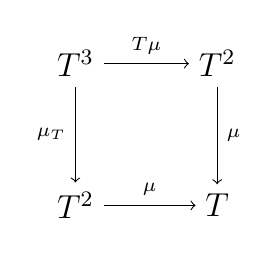
\begin{tikzpicture}
    \node (a) at (0,1.8) {\large $T^{3}$}; \node (b) at (1.8,1.8) {\large $T^{2}$};
    \node (c) at (0,0) {\large $T^{2}$};\node (d) at (1.8,0) {\large $T$};
    \draw[auto,->] (a) -- node {$\scriptstyle T\mu$} (b); \draw[auto,<-] (c) -- node {$\scriptstyle \mu_{T}$} (a);
    \draw[auto,->] (b) -- node {$\scriptstyle \mu$} (d); \draw[auto,->] (c) -- node {$\scriptstyle \mu$} (d);
  \end{tikzpicture}\,\,%
  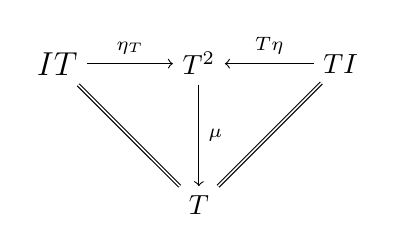
\begin{tikzpicture}
    \node (a) at (0,1.8) {\large $IT$}; \node (b) at (1.8,1.8) {$T^{2}$}; \node (c) at (3.6,1.8) {$TI$};
    \node (d) at (1.8,0) {$T$};
    \draw[double] (a) -- node {$$} (d); \draw[double] (c) -- node {$$} (d);
    \draw[auto,->] (a) -- node {$\scriptstyle \eta_{T}$} (b); \draw[auto,<-] (b) -- node {$\scriptstyle T\eta$} (c);
    \draw[auto,->] (b) -- node {$\scriptstyle \mu$} (d);
  \end{tikzpicture}
\end{dfn}






%
%
\end{document}